\documentclass{article}
\usepackage{graphicx} % Required for including images

\begin{document}

\title{CS 301 Assignment 2\\[0.5cm]\large Student ID: 200482797}
\author{Owen Monus}
\date{March 8th, 2024}

\maketitle

\begin{enumerate}
    \raggedright
    \item Consider two different machines, with two different instruction sets, both of which have a
    clock rate of 200 MHz. The following measurements are recorded on the two machines running a given
    set of programs. Determine the effective CPI, MIPS rate, and execution time for each machine.
        
    \begin{table}[htbp]
        \centering
        \renewcommand{\arraystretch}{2}
        \caption{Equations for Machines \(A\) and \(B\)}
        \label{tab:equations}
        \begin{tabular}{c|c}
            Machine \(A\) & Machine \(B\) \\
            \hline
            \( CPI = \frac{\sum_{i=1}^{n}{CPI_i \times I_i}}{{n}} \) & 
            \( CPI = \frac{\sum_{i=1}^{n}{CPI_i \times I_i}}{{n}} \) \\
            \( CPI = \frac{8 \times 1 + 4 \times 3 + 2 \times 4 + 4 \times 3}{18} \) & 
            \( CPI = \frac{10 \times 1 + 8 \times 2 + 2 \times 4 + 4 \times 3}{24} \) \\
            \( CPI = \frac{40}{18} \approx 2.22 \) & \( CPI = \frac{46}{24} \approx 1.92\) \\
            \hline
            \( MIPS = \frac{f \times 10^6}{CPI \times 10^6} \) & 
            \( MIPS = \frac{f \times 10^6}{CPI \times 10^6} \) \\
            \( MIPS = \frac{200 \times 10^6}{2.22 \times 10^6} \) & 
            \( MIPS = \frac{200 \times 10^6}{1.92 \times 10^6} \) \\
            
            \( MIPS \approx 90.1 \) & 
            \( MIPS \approx 104.2 \) \\
            \hline
            \( T = CPI \times \frac{1}{f} \times I_c \) & 
            \( T = CPI \times \frac{1}{f} \times I_c \) \\
            \( T = 2.22 \times \frac{1}{200 \times 10^6} \times 18,000,000 \) & 
            \( T = 1.92 \times \frac{1}{200 \times 10^6} \times 24,000,000 \) \\
            \( T = 0.1998 \) & 
            \( T = 0.2304\) \\
        \end{tabular}
    \end{table}

    \pagebreak
    
    \raggedright
    \item Consider the following code:
    \begin{verbatim}
for (i = 0; i < 20; i++)
    for (j = 0; j < 10; j++)
        a[i] = a[i] * j
    \end{verbatim}
    \begin{enumerate}
        \item Give one example of the spatial locality in the code. 
        \newline An example of spatial locality in this code can be seen in the array $a$. 
        The data in $a$ is stored linearly and accessed sequentially.
        \item Give one example of the temporal locality in the code.
        \newline An example of temporal locality in this code can be seen in the line that modifies $a$.
        This line of code is repetitively accessed in the for loops, lending temporal locality to the instruction
        and the data accessed in the array $a$
    \end{enumerate}

    \item What do you mean by CPI, average CPI, and MIPS? Derive the formula for MIPS, in terms of clock frequency and average CPI.
    \paragraph{} CPI stands for cycles per instruction, which details how many fetch-execute cycles are needed to execute a single instruction. Average CPI, or average cycles per instruction represents the mean number of cycles for a specified program. Average CPI takes into account the total amount of instructions executed in a program, the amount of each type of instruction, and the CPI of each instruction individually. MIPS is a formula to determine the millions of instructions per second of a specified machine running a specified program.
    
    \paragraph{} The textbook gives the formula for MIPS, in terms of clock frequency and average CPI as follows:
    \( {MIPS} = \frac{f}{CPI \times 10^6}\)

    \pagebreak
    \item Explain the fetch-execute cycle of an instruction using a Finite State Machine (FSM).
    \centering
    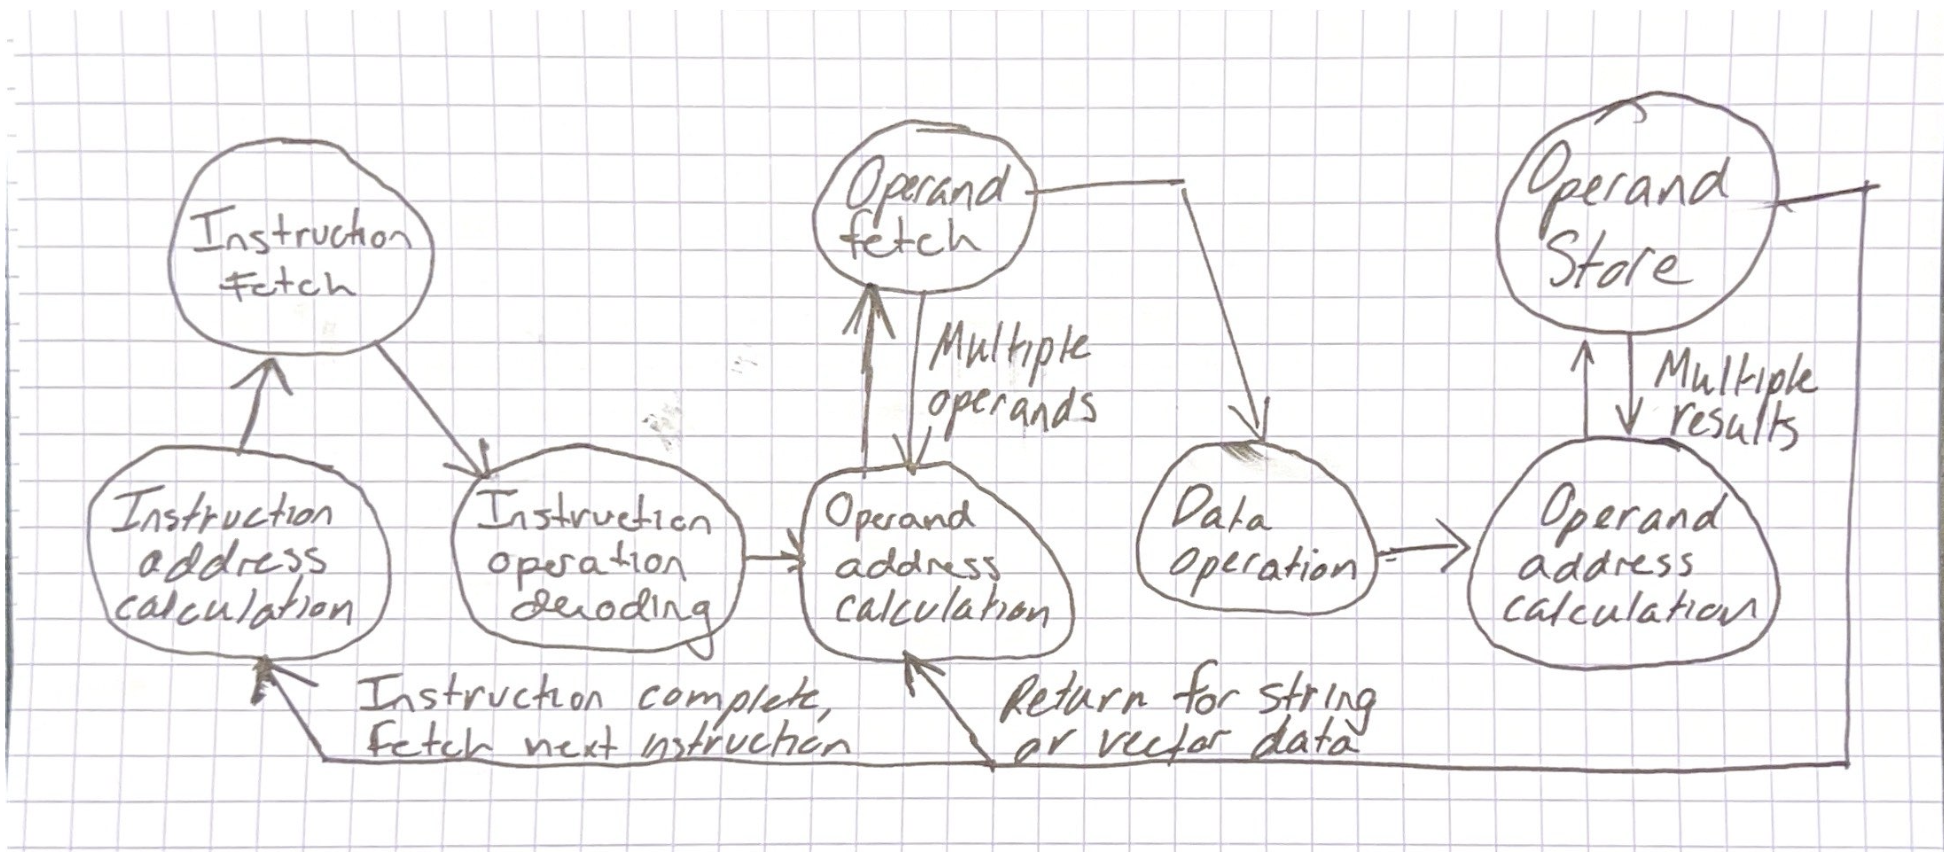
\includegraphics[width=\textwidth]{fsm.png} % Replace example-image.jpg with your image filename
    \raggedright
    \paragraph{} States in the upper part of the figure involve transfer of data between processor and memory or I/O
    module. States in the lower part of the diagram involve internal processor operations.
    The operand address caclulation state appears twice, because an instruction may involve a read, a write, or both.
    
    \pagebreak
    \item Consider these terms: instruction spatial locality, instruction temporal locality, data spatial
    locality, data temporal locality. Match each of these terms to one of the following definitions:

    \begin{table}[htbp]
        \centering
        \renewcommand{\arraystretch}{2}
        % \begin{tabular}{cc}
        \begin{tabular}{p{7cm}|p{2cm}} % Adjust the width as needed
        % \hline
        (a) Locality is quantified by computing the average distance (in terms of number of operand memory accesses) between two consecutive accesses to the same address, for every unique address in the program. The evaluation is performed in four distinct window sizes, analogous to cache block sizes. 
        & instruction temporal locality \\
        (b) Locality metric is quantified by computing the average distance (in terms of number of instructions) between two consecutive accesses to the same static instruction, for every unique static instruction in the program that is executed at least twice.
        & instruction spatial locality \\
        (c) Locality for operand memory accesses is characterized by the ratio of the locality metric for window sizes mentioned in (a).
        & data temporal locality. \\
        (d) Locality is characterized by the ratio of the locality metric for the window sizes mentioned in (b).
        & data spatial locality \\
        % Row 3, Column 1 & Row 3, Column 2 & Row 3, Column 3 \\
        \end{tabular}
        \label{tab:wrapped_table}
    \end{table}
\end{enumerate}

\end{document}